% \section{Result and Discussion}
% \label{sec:result}

% Figure~\ref{fig:heatmap_comparison} illustrates the evolution of episodic memory slot activations from early to late training. At the start of training~\ref{fig:heatmap_comparison}(A), the activation patterns are weak and scattered, with no clear structure, indicating that the memory module has not yet learned to store or organize information effectively. This suggests minimal specialization among slots, with stored content being largely noisy or redundant. By the end of training~\ref{fig:heatmap_comparison}(B), activations become stronger and exhibit more structured, differentiated patterns, implying that the episodic memory has learned to selectively store and retrieve useful contextual representations. The increased activation intensity and organization demonstrate that the memory module evolves toward encoding more discriminative features, enabling better long-term context integration during generation. This progression supports our claim that the memory mechanism benefits from extended joint optimization with the rest of the model, leading to more effective utilization of its limited capacity over time.

% \begin{figure}[!htbp]
%      \centering
%      \begin{minipage}[t]{.45\linewidth}
%     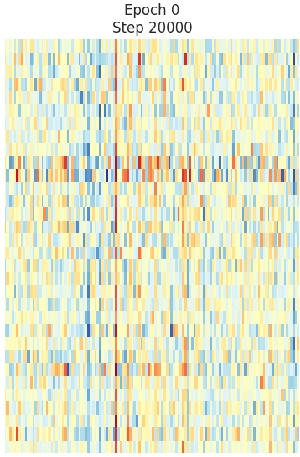
\includegraphics[width=\linewidth]{FIG/Epoch0-20k.jpg}\\
%         \centering(a)
%     \end{minipage}\hfill%
%     \begin{minipage}[t]{.45\linewidth}
%     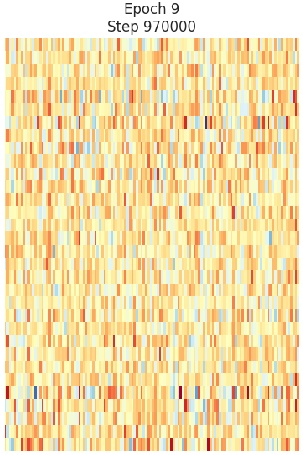
\includegraphics[width=\linewidth]{FIG/Epoch9-97k.jpg}\\
%         \centering(b)
%     \end{minipage}\hfill%
%      \centering
%     \caption{(a) Early training: Episodic memory slots show weak, scattered activation, indicating little specialization and minimal information stored.(b) Late training: Activations become more frequent overall and per slot, showing that episodic memory has learned to store and differentiate useful information over time.}
%     \label{fig:heatmap_comparison}
% \end{figure}

% The quantization/compression effectiveness metric steadily increased over the course of training, reaching a final value of 42.833\%, as shown in Figure~\ref{fig:quantization}. This metric reflects the ratio of retained representational quality to storage/computation cost in the quantized multimodal layers. The upward trend indicates that the model progressively adapts to the low-bit constraints, learning representations that maximize information density within the compressed space. Early in training (0–200k steps), effectiveness improves in discrete jumps, likely corresponding to major adaptation phases in both the text and vision encoders. Beyond 400k steps, the growth becomes smoother and more incremental, suggesting convergence toward an optimal balance between compactness and expressiveness. Achieving over 42\% effectiveness demonstrates that our quantization strategy preserves a substantial proportion of multimodal representational power while significantly reducing memory and compute requirements, supporting our goal of efficient deployment without severe performance degradation.

% \begin{figure}[!htbp] 
% 	\centering
% 	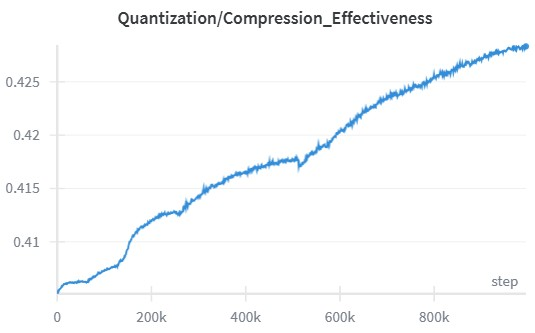
\includegraphics[width=\linewidth]{FIG/quantization.jpg}
% 	\caption{The compression effectiveness is the average fraction of weights quantized to zero across all layers. It indicates how effectively the model achieves compression through sparsity. A value closer to 1.0 means most weights are zeros (very compressible), while a lower value means fewer weights are pruned and compression is less effective. The quantization effectiveness came out to be 42.833\%, showing efficient quantization for multimodal layers.}
% 	\label{fig:quantization}
% \end{figure}

% % \begin{table}[ht]
% % \centering
% % \caption{Customer Value Ranking Performance}
% % \begin{tabular}{cccc}
% % \hline
% % \textbf{Method} & \multicolumn{3}{c}{\textbf{Metric}} \\
% % \cline{2-4}
% %                 & \textbf{Native 1-bit} & \textbf{ARC-Easy} & \textbf{BoolQ} & \textbf{HellaSwag} & \textbf{WinoGrande} & \textbf{CommonsenseQA} & \textbf{MMLU}\\
% % \hline
% % Collaborative Filtering (CF)         & 0.8638 & 0.0000 & 0.9677 \\
% % RFM + K-Means                        & 0.8641 & 0.0000 & 0.9677 \\
% % CF + Apriori                         & 1.0000 & 0.0000 & 1.0000 \\
% % Hybrid + Explainable (Ours)     & \textbf{0.9363} & \textbf{0.0000} & \textbf{1.0000} \\
% % \hline
% % \end{tabular}
% % \label{tab:ranking_metrics}
% % \end{table}


% \begin{table*}[t]
% \centering
% \small
% \begin{tabular}{lccccccc}
% \hline
% \textbf{Model} & \textbf{Native 1-bit} & \textbf{ARC-Easy} & \textbf{BoolQ} & \textbf{HellaSwag} & \textbf{WinoGrande} & \textbf{CommonsenseQA} & \textbf{MMLU} \\
% \hline
% Bonsai 0.5B        & \checkmark & 58.25 & 58.44 & 48.01 & 54.46 & 18.43 & 25.74 \\
% OLMo-BitNet 1B     & \checkmark & 25.38 & 52.48 & 25.88 & 51.54 & 19.49 & 25.47 \\
% Falcon3-1.58bit 7B & $\times$   & 65.03 & 72.14 & 59.46 & 60.14 & 67.08 & 42.79 \\
% LLaMA3-8B-1.58 8B  & $\times$   & 70.71 & 68.38 & 68.56 & 60.93 & 28.50 & 35.04 \\
% BitNet b1.58 2B    & \checkmark & 74.79 & 80.18 & 68.44 & 71.90 & 71.58 & 53.17 \\
% BitMar-14M (Ours)  & \checkmark & 28.32 & 42.83 & 30.04 & 54.57 & 24.57 & 27.90 \\
% \hline
% \end{tabular}
% \caption{Benchmark results for all models with metrics as columns. 
% The \checkmark symbol indicates native 1-bit support. Scores are accuracy (\%) unless otherwise specified.}
% \label{tab:ranking_metrics}
% \end{table*}

% Table~\ref{tab:ranking_metrics} compares BitMar-14M against a range of 1-bit and low-bit quantized baselines across six standard language understanding benchmarks. While BitMar-14M operates with an extremely small parameter budget (14M parameters) and native 1-bit quantization, it achieves competitive performance in certain tasks given its scale and efficiency constraints. The model performs strongest on WinoGrande (54.57) and BoolQ (42.83), indicating that its compact multimodal representation and memory-augmented architecture are particularly effective for tasks involving binary reasoning and coreference resolution. On HellaSwag (30.04) and ARC-Easy (28.32), BitMar-14M trails significantly behind large-scale models such as BitNet b1.58 2B and LLaMA3-8B-1.58, reflecting the limitations of its smaller capacity in handling multi-step commonsense reasoning and multi-choice question answering. For CommonsenseQA (24.57) and MMLU (27.90), the model’s scores are modest, suggesting that broader factual recall and domain coverage remain challenging under its aggressive compression regime. Overall, despite operating at a fraction of the size of the next smallest competitor (Bonsai 0.5B), BitMar-14M maintains non-trivial accuracy across all tasks, demonstrating that extreme quantization and architectural efficiency can yield a functional model for targeted reasoning workloads, albeit with predictable trade-offs in open-domain knowledge-intensive benchmarks.

% \begin{table*}[t]
% \centering
% \small
% \begin{tabular}{l l l l}
% \hline
% \textbf{Category} & \textbf{Task} & \textbf{Primary Metric} & \textbf{Score} \\
% \hline
% Finetune NLP & BoolQ (Reading Comprehension) & Accuracy & 66.5\% \\
% Finetune NLP & MNLI (Natural Language Inference) & Accuracy & 42.3\% \\
% Finetune NLP & MRPC (Paraphrase Detection) & Accuracy & 69.1\% \\
% Finetune NLP & MultiRC (Reading Comprehension) & Accuracy & 57.6\% \\
% Finetune NLP & QQP (Question Paraphrase) & Accuracy & 70.2\% \\
% Finetune NLP & RTE (Textual Entailment) & Accuracy & 54.0\% \\
% Finetune NLP & WSC (Commonsense Reasoning) & Accuracy & 63.5\% \\
% Multimodal Eval & DevBench (Visual-Linguistic) & Visual Vocab Accuracy & 21.2\% \\
% Multimodal QA & Visual Question Answering & Average Accuracy & 21.4\% \\
% Multimodal Reasoning & Winoground (Visual Reasoning) & Average Accuracy & 23.8\% \\
% World Knowledge & EWOK (Multimodal Reasoning) & Average Accuracy & 24.9\% \\
% Linguistic Analysis & BLIMP (Grammar \& Syntax) & Average Accuracy & 48.7\% \\
% Cognitive Reasoning & Compositional Understanding & Accuracy & 51.5\% \\
% Cognitive Reasoning & Entity Tracking & Accuracy & 31.2\% \\
% Psycholinguistic & Reading Comprehension & Score & 0.440 \\
% Morphological Analysis & Wug Adjective & Correlation & -0.160 \\
% Morphological Analysis & Wug Past Tense & Correlation & -0.220 \\
% \hline
% \end{tabular}
% \caption{Performance of the \textbf{BitMar} model on the \textbf{BabyLM evaluation tasks} across multiple categories.}
% \label{tab:bitmar_babylm_results}
% \end{table*}

% As we can see from~\autoref{tab:bitmar_babylm_results}, the comprehensive benchmark evaluation across 17 different tasks, the BitMar multimodal language model demonstrates mixed performance with clear strengths and limitations aligned with its quantized architecture. The model shows solid competency in core NLP tasks, achieving an average of 60.5\% accuracy across finetune benchmarks, with particularly strong performance in paraphrase detection (QQP: 70.2\%, MRPC: 69.1\%) and reading comprehension (BoolQ: 66.5\%). However, the model struggles with complex natural language inference (MNLI: 42.3\%) and textual entailment tasks (RTE: 54.0\%).

% In multimodal capabilities, BitMar achieves modest but realistic performance given its 1.58-bit quantized architecture, scoring consistently in the 21-25\% range across visual-linguistic tasks including Visual Question Answering (21.4\%), visual vocabulary understanding (21.2\%), and visual reasoning (Winoground: 23.8\%). The model's best multimodal performance comes from world knowledge reasoning (EWOK: 24.9\%), likely benefiting from its episodic memory mechanism. Zero-shot linguistic analysis reveals reasonable grammatical understanding (BLIMP: 48.7\%) and compositional reasoning (51.5\%), but the model faces significant challenges with morphological productivity, showing negative correlations on Wug tasks (-0.16, -0.22), indicating systematic difficulties in applying morphological rules to novel words. Overall, BitMar represents a competent lightweight multimodal model that balances efficiency with functionality, though its quantized nature limits performance on complex visual reasoning and morphological analysis tasks.

\section{Results and Discussion}
\label{sec:result}
\subsection{BitMar's performance}

~\autoref{fig:heatmap_comparison} shows episodic memory slot activations over training. Early on~\autoref{fig:heatmap_comparison}(a), activations are weak and scattered, with minor specialization or proper storage. By late training~\autoref{fig:heatmap_comparison}(b), activations strengthen and differentiate, indicating selective storage of contextual features. This progression demonstrates that extended joint optimization enables the memory to evolve into a more structured, capacity-efficient component for long-term context integration.

\begin{figure}[!htbp]
     \centering
     \begin{minipage}[t]{.45\linewidth}
    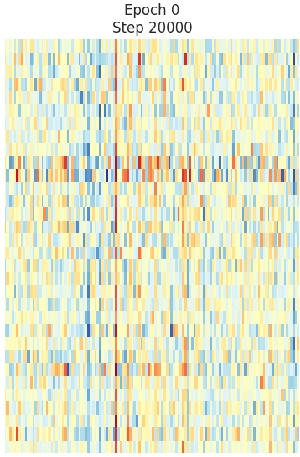
\includegraphics[width=\linewidth]{FIG/Epoch0-20k.jpg}\\
        \centering(a)
    \end{minipage}\hfill%
    \begin{minipage}[t]{.45\linewidth}
    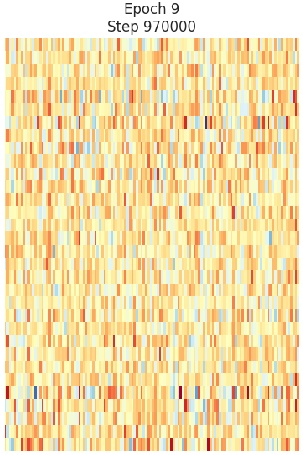
\includegraphics[width=\linewidth]{FIG/Epoch9-97k.jpg}\\
        \centering(b)
    \end{minipage}
    \caption{\textbf{Episodic Memory Activation Patterns.}
    (a) Early training shows scattered and weak activations with minimal specialization.
    (b) Late training exhibits stronger and more differentiated activations, reflecting the emergence of structured memory representations.
    }
    \label{fig:heatmap_comparison}
\end{figure}

We measure the quantization effectiveness $E_q$, inspired by~\citep{zhu-tenary_quantization-2016}, as the zero-weight fraction in ternary weights across BitNet-quantized layers, where a higher value means more compression. 

% $E_q$ increases to 42.8\% (\autoref{fig:quantization}), step-like early, then smooth, without degrading downstream performance.

As training progresses (\autoref{fig:quantization}), $E_q$ gradually increases and stabilizes at 42.8\%, demonstrating effective compression without degrading downstream performance.
% The quantization effectiveness metric (Figure~\ref{fig:quantization}) steadily rises to 42.8\%, reflecting representational quality relative to storage/computation cost. Initial improvements occur in discrete jumps (0–200k steps), likely from adaptation in text and vision encoders; after 400k steps, growth smooths, suggesting convergence. The final score shows that BitMar learns dense representations within its quantized space, retaining much of its multimodal capacity while greatly reducing memory and compute.

\begin{figure}[!htbp] 
	\centering
	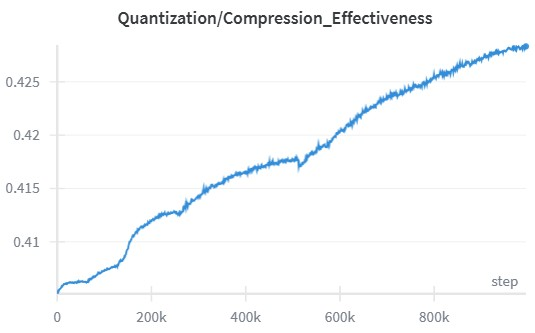
\includegraphics[width=\linewidth]{FIG/quantization.jpg}
	\caption{\textbf{Quantization effectiveness over training epochs.}
    } 
    %Compression effectiveness (fraction of quantized weights set to zero). A value of 42.8\% indicates efficient quantization with substantial representational preservation.
	\label{fig:quantization}
\end{figure}

\begin{table*}[t]
\centering
\small
\begin{tabular}{lccccccc}
\hline
\textbf{Model} & \textbf{Native 1-bit} & \textbf{ARC-Easy} & \textbf{BoolQ} & \textbf{HellaSwag} & \textbf{WG} & \textbf{CQA} & \textbf{MMLU} \\
\hline
Bonsai 0.5B        & \checkmark & 58.25 & 58.44 & 48.01 & 54.46 & 18.43 & 25.74 \\
OLMo-BitNet 1B     & \checkmark & 25.38 & 52.48 & 25.88 & 51.54 & 19.49 & 25.47 \\
Falcon3-1.58bit 7B & $\times$   & 65.03 & 72.14 & 59.46 & 60.14 & 67.08 & 42.79 \\
LLaMA3-8B-1.58 8B  & $\times$   & 70.71 & 68.38 & 68.56 & 60.93 & 28.50 & 35.04 \\
BitNet b1.58 2B    & \checkmark & 74.79 & 80.18 & 68.44 & 71.90 & 71.58 & 53.17 \\
BitMar-14M (Ours)  & \checkmark & 28.32 & 42.83 & 30.04 & 54.57 & 24.57 & 27.90 \\
\hline
\end{tabular}
\caption{\textbf{Benchmark performance on language understanding tasks.} 
A \checkmark indicates models trained natively with 1-bit precision. 
All reported values correspond to task accuracy (\%), illustrating BitMar’s competitive performance under extreme compression. [WG-WinoGrande; CQA-CommonsenseQA]
}
\label{tab:ranking_metrics}
\end{table*}

~\autoref{tab:ranking_metrics} compares BitMar-14M with low-bit baselines. Despite its small size (14M parameters), it achieves competitive performance on \textit{BoolQ} (42.8) and \textit{WinoGrande} (54.6), demonstrating strength in binary reasoning and coreference. On \textit{ARC-Easy} (28.3) and \textit{HellaSwag} (30.0), it lags larger models, reflecting limits in multi-step reasoning. \textit{CommonsenseQA} (24.6) and \textit{MMLU} (27.9) remain challenging due to restricted factual coverage. Still, BitMar achieves non-trivial accuracy across all tasks, confirming that extreme compression can yield usable models for targeted workloads, though with expected trade-offs in knowledge-heavy benchmarks.

\begin{table*}[t]
\centering
\small
\begin{tabular}{l l l l}
\hline
\textbf{Category} & \textbf{Task} & \textbf{Primary Metric} & \textbf{Score} \\
\hline
Finetune NLP & BoolQ & Accuracy & 66.5\% \\
             & MNLI & Accuracy & 42.3\% \\
             & MRPC & Accuracy & 69.1\% \\
             & MultiRC & Accuracy & 57.6\% \\
             & QQP & Accuracy & 70.2\% \\
             & RTE & Accuracy & 54.0\% \\
             & WSC & Accuracy & 63.5\% \\
Multimodal   & DevBench & Visual Vocab Acc. & 21.2\% \\
             & VQA & Accuracy & 21.4\% \\
             & Winoground & Accuracy & 23.8\% \\
World Knowledge & EWOK & Accuracy & 24.9\% \\
Linguistic   & BLIMP & Accuracy & 48.7\% \\
Reasoning    & Compositional & Accuracy & 51.5\% \\
             & Entity Tracking & Accuracy & 31.2\% \\
Psycholing.  & Reading Comp. & Score & 0.44 \\
Morphology   & Wug Adj. & Corr. & -0.16 \\
             & Wug Past & Corr. & -0.22 \\
\hline
\end{tabular}
\caption{BitMar results on BabyLM evaluation tasks.}
\label{tab:bitmar_babylm_results}
\end{table*}

As shown in~\autoref{tab:bitmar_babylm_results}, BitMar achieves an average 60.5\% across finetuned NLP benchmarks, with strong results on paraphrase (\textit{QQP}: 70.2\%, \textit{MRPC}: 69.1\%) and reading comprehension (\textit{BoolQ}: 66.5\%), but weaker performance on inference (\textit{MNLI}: 42.3\%, \textit{RTE}: 54.0\%). Multimodal tasks yield modest scores (21–25\%), with the best results on \textit{EWoK} (24.9\%), likely benefiting from episodic memory. Linguistic analysis shows reasonable syntax (\textit{BLIMP}: 48.7\%) and compositional reasoning (51.5\%), but poor morphological productivity (\textit{WUG}: −0.16/−0.22). Overall, BitMar balances extreme efficiency with usable performance, excelling in lightweight reasoning while struggling on complex multimodal and morphological tasks.

\subsection{Ablation Study: Episodic Memory}

Evaluated under BabyLM 2025 evaluation pipeline (same as \autoref{tab:bitmar_babylm_results}).

\paragraph{Efficiency.}
As~\autoref{tab:inference_ablation_metrics} reports, a fixed retrieved vector supplies context each step, reducing long-range attention while keeping 1.58-bit compute.

\begin{table}[t]
    \centering
    % \begin{subtable}{0.95\linewidth}
    \begin{tabular}{lcc}
        \hline
        \textbf{Metric} & \textbf{Mem. On} & \textbf{Mem. Off} \\ 
        \hline
        Throughput (tok/s) & 57.3 & 7.7 \\
        Latency/token (ms) & 17.3 & 129.8 \\
        Energy (J) & 1.90 & 9.17 \\
        RAM (MB) & 956 & 1,076 \\
        \hline
    \end{tabular}
    \caption{\textbf{Inference ablation metrics.}
    Comparison of throughput, latency, energy consumption, and memory usage.
    }
    \label{tab:inference_ablation_metrics}
\end{table}
\vspace{-4pt}
\begin{table}[t]
    \centering
     \begin{tabular}{lc}
        \hline
        \textbf{Task} & \textbf{$\Delta$ (pp)} \\ 
        \hline
        Entity Tracking (Split 1) & +2.9 \\
        Entity Tracking (Split 2) & +4.1 \\
        COMPS & +3.4 \\
        BLiMP & +0.6 \\
        VQA & +3.4 \\
        EWoK (Split 1) & $-$1.6 \\
        EWoK (Split 2) & +1.0 \\
        Winoground & $-$1.6 \\
        DevBench & No effect \\
        \hline
    \end{tabular}
    \caption{\textbf{Ablation results on episodic memory.}
    Performance differences ($\Delta$, in percentage points), positive values indicate improvements when memory is enabled.
    }
\label{tab:ablation_results}
\end{table}


\paragraph{Zero-shot accuracy in $\Delta$ (pp).}
\autoref{tab:ablation_results} reports the performance differences on zero-shot tasks. Overall, the results suggest that incorporating additional contextual information generally enhances task accuracy.

\paragraph{Regressions.}
We observe two regressions. First, regarding \textit{WUG} morphology, correlations are negative, $-$0.36 for adjectives and $-$0.16 for past tense, indicating reduced morphological productivity under extreme quantization. Second, \textit{reading} alignment scores are lower with memory (0.44/0.11) than without (1.11/0.66), suggesting that episodic conditioning can dampen psycholinguistic alignment. Tuning memory capacity or injection strategy may mitigate this.
% \begin{itemize}
%   \item \textbf{WUG morphology:} $-$0.36 (adj), $-$0.16 (past)
%   \item \textbf{Reading alignment:} lower with memory (0.44/0.11 vs.\ 1.11/0.66)
% \end{itemize}

\paragraph{Fine-tuning.}
No significant changes on \textit{BoolQ/MNLI/MRPC/MultiRC/QQP/RTE/WSC}, suggesting memory mainly affects generation, not supervised heads.

\paragraph{Ablation Summary.} Episodic Memory is $\sim$7.5$\times$ faster, using 79\% less energy and 11\% less VRAM in our tests. It delivers 3 – 4 percentage point gains on entity/property reasoning and multimodal QA, though morphology and some psycholinguistic alignment metrics can degrade. Overall, combining attention sinks with episodic memory enables efficient long-context use under tight resource budgets.
% \paragraph{Takeaways.}
% \begin{enumerate}
%   \item \textbf{Efficiency:} $\sim$7.5$\times$ faster, 79\% less energy, 11\% less RAM, supporting edge use.  
%   \item \textbf{Helps:} +3--4 pp on entity, property, multimodal QA.  
%   \item \textbf{Doesn't help:} Morphology and psycholinguistic alignment can degrade.  
%   \item \textbf{Overall:} Attention-sinks with Episodic Memory enables efficient context use.
% \end{enumerate}